% exercise sheet with header on every page for math or close subjects
\documentclass[12pt]{article}
\usepackage[utf8]{inputenc} 
\usepackage{latexsym} 
\usepackage{multicol}
\usepackage{fancyhdr}
\usepackage{amsfonts} 
\usepackage{amsmath}
\usepackage{amssymb}
\usepackage{enumerate}
\usepackage{listings}
\usepackage{graphicx}
\usepackage{hyperref}

% Shortcuts for bb, frak and cal letters
\newcommand{\E}{\mathbb{E}}
\newcommand{\V}{\mathbb{V}}
\renewcommand{\P}{\mathbb{P}}
\newcommand{\N}{\mathbb{N}}
\newcommand{\R}{\mathbb{R}}
\newcommand{\C}{\mathbb{C}}
\newcommand{\Z}{\mathbb{Z}}
\newcommand{\Pfrak}{\mathfrak{P}}
\newcommand{\Pfrac}{\mathfrak{P}}
\newcommand{\Bfrac}{\mathfrak{P}}
\newcommand{\Bfrak}{\mathfrak{B}}
\newcommand{\Fcal}{\mathcal{F}}
\newcommand{\Ycal}{\mathcal{Y}}
\newcommand{\Bcal}{\mathcal{B}}
\newcommand{\Acal}{\mathcal{A}}

% formating
\topmargin -1.5cm 
\textheight 24cm
\textwidth 16.0 cm 
\oddsidemargin -0.1cm

% Fancy Header on every Page
\pagestyle{fancy}
\lhead{\textbf{Pattern and Speech Recognition}}
\rhead{Daniel Schäfer (2549458)\\ Christian Bohnenberger (2548364) \\ Dominik Weber (2548553)}
\renewcommand{\headrulewidth}{1.2pt}

\setlength{\headheight}{45pt} 

\begin{document}
\pagenumbering{gobble}

% TODO set the number of the exercise sheet here!
\setcounter{section}{8}
\setcounter{subsection}{0}

\subsection{ }

\begin{enumerate}[a)]
\item
\begin{itemize}
	\item $s_1[0]= 0.5 * 3 = 1.5 $
	\item $s_1[1]= 0.5 * 3 + 0.5 * 1 = 2 $
	\item $s_1[2]= 0.5 * 1 + 0.5 * 8 = 4.5 $	
	\item $s_1[3]= 0.5 * 8 + 0.5 * 6 = 7 $
	\item $s_1[4]= 0.5 * 6 + 0.5 * 3 = 4.5 $	
	\item $s_1[5]= 0.5 * 3 + 0.5 * 9 = 6 $
	\item $s_1[6]= 0.5 * 9 + 0.5 * 5 = 7 $
	\item $s_1[7]= 0.5 * 5 + 0.5 * 1 = 3 $
	\item $s_1[8]= 0.5 * 1 = 0.5 $
\end{itemize}
$s_1$=\begin{tabular}{|c|c|c|c|c|c|c|c|c|}
\hline
1.5 & 2 & 4.5 & 7 & 4.5 & 6 & 7 & 3 & 0.5\\ \hline
\end{tabular}
\item
computation as in a.) \\
$s_2=$\begin{tabular}{|c|c|c|c|c|c|c|c|c|c|}
\hline
0.75 & 1.75 & 3.25 & 5.75 & 5.75 & 5.25 & 6.5 & 5 & 1.75 & 0.25\\ \hline
\end{tabular}

\item
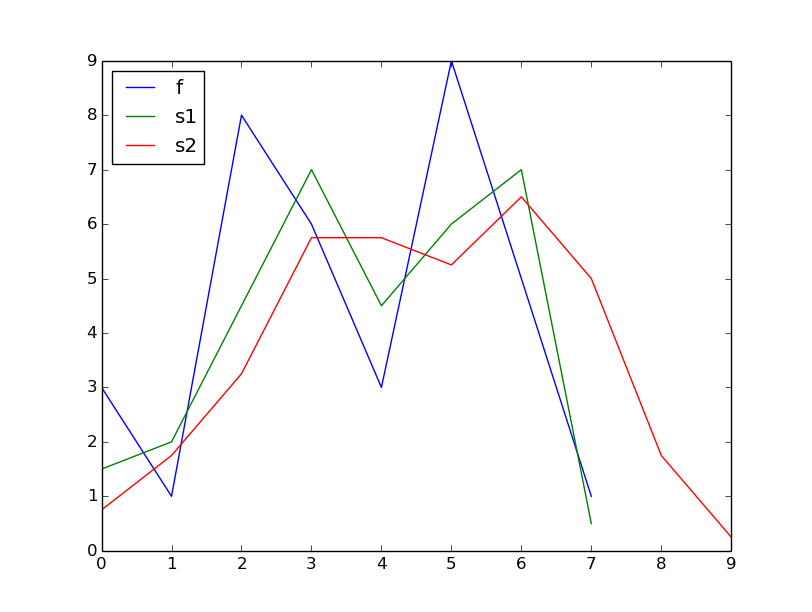
\includegraphics[scale=0.4]{plot81c.png}
The outcome increases the size by 1 every times we use convolution. Furthermore, we can see the values on the edges are very small. And they will be be smaller every times we apply convolution. The big gap between the values in the middle which is given in $f$ is decreased every times convolution is applied. If we apply convolution $n$-times and $n \rightarrow \infty$ we get the values in the middle at about the same value, whereas the values next on the edges are close to 0. In the end the the amplitude will be flattened.

\item
\begin{itemize}
	\item $k'[0]=0.25$
	\item $k'[0]=0.5$
	\item $k'[0]=0.25$\\
	$\Rightarrow k'= $\begin{tabular}{|c|c|c|}
	\hline 0.25 & 0.5 & 0.25 \\ \hline
	\end{tabular}
	\item $s_3[0]= 0.25*3= 0.75$
	\item $s_3[1]= 0.25*1+0.5*3=1.75$
	\item $s_3[2]= 0.25*8+0.5*1+0.25*3=3.25$
	\item \dots \\
	$\Rightarrow s_3=$
	\begin{tabular}{|c|c|c|c|c|c|c|c|c|c|}
		\hline
		0.75 & 1.75 & 3.25 & 5.75 & 5.75 & 5.25 & 6.5 & 5 & 1.75 & 0.25\\ \hline
	\end{tabular}
\end{itemize}

\item 
\begin{itemize}
	\item $s_2$ and $s_3$ are equal that means $(f*k)*k=f*(k*k)$
	\item associativity seems to be fullfilled by convolution
	\item Proof:\\
	We want to show: $(f*g)*h=f*(g*h)$:\\
	$$((f*g)*h)(t) =^{Definition} \int (f*g)(a)*h(t-a) da $$
	$$ =^{Definition} \int (\int f(b)*g(a-b) db)*h(t-a) da $$
	$$=^{Definition}\int \int f(b)*g(a-b)*h(t-a) db~ da $$
	$$=^{Fubini} \int \int f(b)*g(a-b)*h(t-a) da~ db$$
	$$=^{Definition} \int f(b) (\int g(a-b)*h(t-a) da) db$$
	$$=^{Definition} \int f(b)(\int g(a) * h((t-b)-a) da) db $$
	$$=^{Definition} \int f(b) (g*h)(t-b) db$$
	$$=^{Definition} (f*(g*h))(t) $$
\end{itemize}
\end{enumerate}
\end{document}
